\section{Results}
\label{sec:results}

\subsection{The main comparison}
\label{sec:results-main}

Table~\ref{tab:main-results} gives the detection rate of every detector on every variant of the committed bake.
The engine's statistics, recomputed here, agree count for count with the committed C13 documents of the product on all six variants (the Wald, absolute-value and rolling-mean flags and the regulatory zone), so the table extends the committed results and does not replace them.
The critical values read from the 10,000 null desk-years at a size of 1\% per statistic are 9.833 for the Wald statistic, 0.9353 for the absolute-value Spearman and 0.9619 for the rolling-mean Spearman; at the Bonferroni split of the family size they are 12.007, 0.9263 and 0.9493.

\begin{table*}[htbp]
\centering
\scriptsize\setlength{\tabcolsep}{3pt}
\caption{Share of the 1,000 replications of each variant of the committed C13 desk bake (case seed 13) that each detector flags, in percent with the 95\% Wilson interval; the three proposed components and the union are calibrated on 10,000 independent null desk-years at a size of 1\% per statistic (family 1\% for the union), the published comparators at 1\% per statistic on the same null, and the regulatory zone and the desk back-test by their own rules. The no-deficiency column is the held-out false-alarm rate.}
\label{tab:main-results}
\resizebox{\textwidth}{!}{%
\begin{tabular}{p{4.1cm}cccccc}
\toprule
Detector & No deficiency & Missing basis & Stale volatility (20 days) & Wrong correlation & Omitted factor & Time misalignment \\
\midrule
Regulatory zone, amber or red & 0.0 (0.0--0.4) & 96.0 (94.6--97.0) & 0.0 (0.0--0.4) & 100.0 (99.6--100.0) & 90.1 (88.1--91.8) & 100.0 (99.6--100.0) \\
KS distance alone, not green & 0.0 (0.0--0.4) & 86.7 (84.5--88.7) & 0.0 (0.0--0.4) & 100.0 (99.6--100.0) & 44.8 (41.7--47.9) & 0.0 (0.0--0.4) \\
\relax KS distance, threshold recalibrated at 1\% & 0.5 (0.2--1.2) & 99.7 (99.1--99.9) & 6.3 (5.0--8.0) & 100.0 (99.6--100.0) & 99.4 (98.7--99.7) & 0.4 (0.2--1.0) \\
\relax Spearman of levels, threshold recalibrated at 1\% & 1.2 (0.7--2.1) & 100.0 (99.6--100.0) & 55.2 (52.1--58.3) & 7.8 (6.3--9.6) & 100.0 (99.6--100.0) & 100.0 (99.6--100.0) \\
Desk back-test over its limit & 0.0 (0.0--0.4) & 56.5 (53.4--59.5) & 0.5 (0.2--1.2) & 95.4 (93.9--96.5) & 6.4 (5.0--8.1) & 0.0 (0.0--0.4) \\
\relax Christoffersen conditional coverage, 97.5\% & 0.8 (0.4--1.6) & 90.0 (88.0--91.7) & 12.7 (10.8--14.9) & 100.0 (99.6--100.0) & 61.3 (58.2--64.3) & 1.1 (0.6--2.0) \\
MZ Wald, OLS covariance & 1.0 (0.5--1.8) & 0.6 (0.3--1.3) & 41.0 (38.0--44.1) & 100.0 (99.6--100.0) & 1.9 (1.2--2.9) & 100.0 (99.6--100.0) \\
MZ Wald on the squared series & 1.3 (0.8--2.2) & 100.0 (99.6--100.0) & 20.0 (17.6--22.6) & 100.0 (99.6--100.0) & 97.7 (96.6--98.5) & 99.1 (98.3--99.5) \\
Ljung--Box on the squared residual & 1.1 (0.6--2.0) & 1.0 (0.5--1.8) & 71.9 (69.0--74.6) & 45.5 (42.4--48.6) & 47.1 (44.0--50.2) & 84.9 (82.5--87.0) \\
MZ Wald, HC3 (proposed) & 0.8 (0.4--1.6) & 0.9 (0.5--1.7) & 14.2 (12.2--16.5) & 100.0 (99.6--100.0) & 0.6 (0.3--1.3) & 100.0 (99.6--100.0) \\
Spearman of absolute values (proposed) & 1.6 (1.0--2.6) & 100.0 (99.6--100.0) & 76.7 (74.0--79.2) & 8.7 (7.1--10.6) & 100.0 (99.6--100.0) & 100.0 (99.6--100.0) \\
Spearman of 20-day rolling means (proposed) & 1.2 (0.7--2.1) & 99.9 (99.4--100.0) & 99.9 (99.4--100.0) & 4.5 (3.4--6.0) & 98.7 (97.8--99.2) & 42.3 (39.3--45.4) \\
\relax Union of the three proposed, family 1\% & 0.9 (0.5--1.7) & 100.0 (99.6--100.0) & 99.9 (99.4--100.0) & 100.0 (99.6--100.0) & 100.0 (99.6--100.0) & 100.0 (99.6--100.0) \\
\bottomrule
\end{tabular}}
\end{table*}


On the stale-volatility desk, the regulatory zone flags none of the 1,000 replications (0.0\%, interval 0.0 to 0.4\%), the Kolmogorov--Smirnov distance alone flags none, the desk back-test flags 0.5\% (0.2 to 1.2\%) and the Christoffersen test 12.7\% (10.8 to 14.9\%).
The union of the three proposed statistics flags 99.9\% (99.4 to 100.0\%), and the rolling-mean statistic alone flags 99.9\% as well.
The comparators that read the dynamics or the scale come between: the Ljung--Box statistic of the squared residual flags 71.9\% (69.0 to 74.6\%), the absolute-value Spearman 76.7\% (74.0 to 79.2\%), the Wald test on the squares 20.0\%, the Wald test with the ordinary covariance 41.0\% (38.0 to 44.1\%) and the same test with the HC3 covariance 14.2\% (12.2 to 16.5\%).
The two regulatory statistics with their thresholds moved to the same 1\% size are informative about where the blind spot lies: the Kolmogorov--Smirnov distance flags 6.3\% and the Spearman correlation of the levels 55.2\%.
A large part of the failure of the regulatory zone on this desk is therefore the position of its thresholds, written for a green limit of 0.80 where the correct model has a mean of 0.992, and the rest is the choice of statistic, since no recalibrated level statistic reaches the rolling mean's 99.9\%.

On the other variants the complement keeps what the regulatory zone has and adds what it lacks.
The union flags the missing-basis, wrong-correlation, omitted-factor and time-misalignment variants in 100.0\% of replications, where the regulatory zone flags 96.0, 100.0, 90.1 and 100.0\%.
The components are not interchangeable.
The rolling-mean statistic flags the wrong-correlation variant in 4.5\% and the time-misalignment variant in 42.3\%, and the absolute-value statistic flags the wrong correlation in 8.7\%; the Wald test flags the missing-basis variant in 0.9\% and the omitted-factor variant in 0.6\%, at its false-alarm rate, as Corollary~\ref{cor:noise} predicts for a basis independent of RTPL.
On the desk with no deficiency the false-alarm rates are 0.9\% (0.5 to 1.7\%) for the union, 1.2\% for the rolling-mean statistic, 1.6\% (1.0 to 2.6\%) for the absolute-value statistic and 0.8\% for the Wald test; with 1,000 held-out desk-years the sampling standard deviation of a rate near 1\% is 0.31 percentage points, so the interval of the absolute-value statistic is compatible with its 1\% size.
Figure~\ref{fig:detection-map} shows the table as a map: the three proposed statistics cover, jointly, the columns that each of them leaves pale.

\begin{figure}[htbp]
\centering
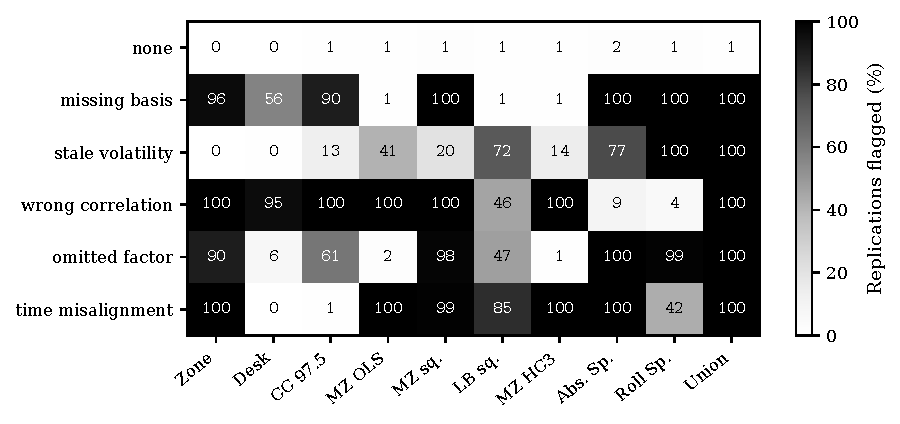
\includegraphics[width=0.92\linewidth]{detection-map}
\caption{Percent of the 1,000 replications of each C13 variant flagged by each detector at its calibrated size, on the committed bake; darker cells are higher rates, and the stale-volatility row is the one the regulatory zone does not flag.}
\label{fig:detection-map}
\end{figure}

\subsection{Stability across independent bakes}
\label{sec:results-repeats}

The committed bake is one draw of 1,000 desk-years per variant.
Table~\ref{tab:repeats} gives the mean and the standard deviation of each rate over five further bakes of 1,000, drawn under other case seeds, with the thresholds unchanged.
The stale-volatility rates are stable: the union flags $99.9\pm0.2$\% and the rolling-mean statistic alone $100.0\pm0.0$\%, the absolute-value statistic $75.3\pm0.7$\%, the Ljung--Box statistic $71.8\pm0.9$\%, the recalibrated Spearman correlation of the levels $56.8\pm0.8$\% and the regulatory zone $0.0\pm0.0$\%.
The false-alarm rate of the union on five fresh null bakes is $1.0\pm0.3$\%, that of the rolling-mean statistic $0.8\pm0.3$\% and that of the absolute-value statistic $1.0\pm0.2$\%, so the 1.6\% of the committed bake for the last is a draw at the upper end of that spread and not a drift.
The weak cells repeat too: the rolling-mean statistic flags the wrong correlation in $4.8\pm0.5$\% and the time misalignment in $42.9\pm0.2$\%.
Across the table the standard deviation over bakes never exceeds 2 percentage points.

\begin{table*}[htbp]
\centering
\scriptsize\setlength{\tabcolsep}{3pt}
\caption{Mean and standard deviation, in percent, of each detector's flag rate over five further independent bakes of 1,000 replications per variant (case seeds 23, 33, 43, 53 and 63), with the thresholds of the calibration null unchanged. The no-deficiency column is the false-alarm rate on five fresh null bakes.}
\label{tab:repeats}
\resizebox{\textwidth}{!}{%
\begin{tabular}{p{4.1cm}cccccc}
\toprule
Detector & No deficiency & Missing basis & Stale volatility (20 days) & Wrong correlation & Omitted factor & Time misalignment \\
\midrule
Regulatory zone, amber or red & $0.0\pm0.0$ & $94.9\pm0.5$ & $0.0\pm0.0$ & $100.0\pm0.0$ & $90.1\pm0.8$ & $100.0\pm0.0$ \\
\relax Spearman of levels, threshold recalibrated at 1\% & $0.9\pm0.3$ & $100.0\pm0.0$ & $56.8\pm0.8$ & $7.8\pm0.8$ & $100.0\pm0.0$ & $100.0\pm0.0$ \\
Desk back-test over its limit & $0.0\pm0.0$ & $58.4\pm1.9$ & $0.6\pm0.2$ & $96.0\pm0.5$ & $6.3\pm1.0$ & $0.0\pm0.0$ \\
\relax Christoffersen conditional coverage, 97.5\% & $0.8\pm0.4$ & $91.2\pm1.3$ & $12.4\pm0.4$ & $100.0\pm0.1$ & $61.5\pm1.6$ & $1.0\pm0.1$ \\
MZ Wald, OLS covariance & $0.8\pm0.4$ & $1.2\pm0.4$ & $38.7\pm1.5$ & $100.0\pm0.0$ & $1.9\pm0.6$ & $100.0\pm0.0$ \\
Ljung--Box on the squared residual & $0.9\pm0.2$ & $0.9\pm0.1$ & $71.8\pm0.9$ & $45.0\pm0.8$ & $50.7\pm1.7$ & $84.4\pm1.1$ \\
MZ Wald, HC3 (proposed) & $0.8\pm0.3$ & $1.1\pm0.3$ & $13.6\pm0.9$ & $100.0\pm0.0$ & $0.9\pm0.4$ & $100.0\pm0.0$ \\
Spearman of absolute values (proposed) & $1.0\pm0.2$ & $100.0\pm0.0$ & $75.3\pm0.7$ & $8.8\pm0.8$ & $100.0\pm0.0$ & $100.0\pm0.0$ \\
Spearman of 20-day rolling means (proposed) & $0.8\pm0.3$ & $99.9\pm0.1$ & $100.0\pm0.0$ & $4.8\pm0.5$ & $98.5\pm0.3$ & $42.9\pm0.2$ \\
\relax Union of the three proposed, family 1\% & $1.0\pm0.3$ & $100.0\pm0.0$ & $99.9\pm0.2$ & $100.0\pm0.0$ & $100.0\pm0.0$ & $100.0\pm0.0$ \\
\bottomrule
\end{tabular}}
\end{table*}


\subsection{The age of the volatility input}
\label{sec:results-lag}

Figure~\ref{fig:mechanism} shows the mechanism on one desk-year of each kind: when the risk model's volatility is twenty days old, the 20-day mean of $|\RTPL|$ follows the 20-day mean of $|\HPL|$ with a delay of the order of the lag.
The correlation of the two rolling means is 0.994 on average on the desks with no deficiency and 0.691 on the stale desks.

\begin{figure}[htbp]
\centering
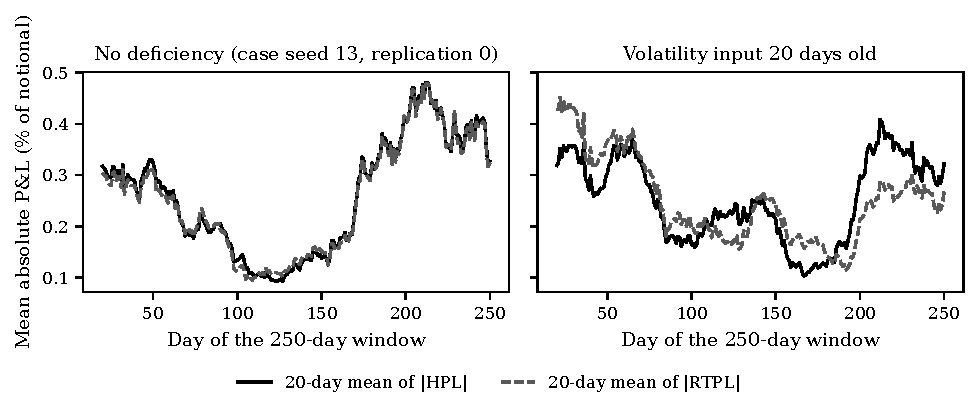
\includegraphics[width=\linewidth]{mechanism}
\caption{Twenty-day rolling means of the absolute hypothetical and risk-theoretical profit and loss of one desk-year with no deficiency (left) and of one desk-year whose risk model uses a volatility twenty days old (right), under the committed generator, in percent of the desk notional.}
\label{fig:mechanism}
\end{figure}

Table~\ref{tab:lag-ladder} and Figure~\ref{fig:power-by-lag} give the rates as the lag grows.
The regulatory zone flags nothing until a lag of 40 days (0.2\%) and flags 5.1\% at 80 days; the desk back-test flags 3.9\% and 13.5\% at the same lags.
The rolling-mean statistic flags 5.7\% at a lag of 2 days, 57.6\% at 5, 97.5\% at 10, 99.9\% at 20 and 100.0\% at 40 and 80 days; the union is a little lower at the short lags (2.9\% and 37.3\% at 2 and 5 days) because the Bonferroni split places each statistic at 0.333\%.
The Ljung--Box statistic rises more slowly (9.0, 26.1, 49.2, 71.9, 82.6 and 86.8\%), the absolute-value statistic is strong from 20 days (76.7\% and above) and weak at 5 and 10 days (4.5 and 25.6\%), and the Wald statistic with the HC3 covariance needs 80 days to flag 45.2\%.
The mean of the Wald statistic goes from 2.05 on the desks with no deficiency to 2.07, 2.54, 3.35, 4.97, 9.04 and 18.78 at the six lags, so the regression component moves in the right direction and slowly, as Proposition~\ref{prop:slope} implies.
The flag rate of the rolling-mean statistic is non-decreasing in the lag over the six lags, so H4 holds on this range.

\begin{table}[htbp]
\centering
\footnotesize
\renewcommand{\arraystretch}{1.1}
\caption{Percent of 1,000 replications flagged, over the 95\% Wilson interval, as the age of the volatility input of the risk model grows from 2 to 80 days (stale-volatility variant, committed seeds; the 20-day row is the committed variant). The first panel holds the regulatory zone and the published comparators, the second the proposed components and their union. Zone is the regulatory zone, Desk the desk back-test limit, CC the Christoffersen conditional coverage, MZ the Mincer--Zarnowitz Wald test with the OLS or HC3 covariance, LB the Ljung--Box test and Sp. the Spearman statistic.}
\label{tab:lag-ladder}
\begin{tabular}{rccccc}
\toprule
Lag (days) & Zone & Desk & CC 97.5 & MZ OLS & LB sq. \\
\midrule
2 & \begin{tabular}[t]{@{}c@{}}0.0\\(0.0--0.4)\end{tabular} & \begin{tabular}[t]{@{}c@{}}0.0\\(0.0--0.4)\end{tabular} & \begin{tabular}[t]{@{}c@{}}1.8\\(1.1--2.8)\end{tabular} & \begin{tabular}[t]{@{}c@{}}5.5\\(4.2--7.1)\end{tabular} & \begin{tabular}[t]{@{}c@{}}9.0\\(7.4--10.9)\end{tabular} \\ \addlinespace[0.8ex]
5 & \begin{tabular}[t]{@{}c@{}}0.0\\(0.0--0.4)\end{tabular} & \begin{tabular}[t]{@{}c@{}}0.0\\(0.0--0.4)\end{tabular} & \begin{tabular}[t]{@{}c@{}}2.8\\(1.9--4.0)\end{tabular} & \begin{tabular}[t]{@{}c@{}}15.1\\(13.0--17.5)\end{tabular} & \begin{tabular}[t]{@{}c@{}}26.1\\(23.5--28.9)\end{tabular} \\ \addlinespace[0.8ex]
10 & \begin{tabular}[t]{@{}c@{}}0.0\\(0.0--0.4)\end{tabular} & \begin{tabular}[t]{@{}c@{}}0.0\\(0.0--0.4)\end{tabular} & \begin{tabular}[t]{@{}c@{}}5.4\\(4.2--7.0)\end{tabular} & \begin{tabular}[t]{@{}c@{}}25.6\\(23.0--28.4)\end{tabular} & \begin{tabular}[t]{@{}c@{}}49.2\\(46.1--52.3)\end{tabular} \\ \addlinespace[0.8ex]
20 & \begin{tabular}[t]{@{}c@{}}0.0\\(0.0--0.4)\end{tabular} & \begin{tabular}[t]{@{}c@{}}0.5\\(0.2--1.2)\end{tabular} & \begin{tabular}[t]{@{}c@{}}12.7\\(10.8--14.9)\end{tabular} & \begin{tabular}[t]{@{}c@{}}41.0\\(38.0--44.1)\end{tabular} & \begin{tabular}[t]{@{}c@{}}71.9\\(69.0--74.6)\end{tabular} \\ \addlinespace[0.8ex]
40 & \begin{tabular}[t]{@{}c@{}}0.2\\(0.1--0.7)\end{tabular} & \begin{tabular}[t]{@{}c@{}}3.9\\(2.9--5.3)\end{tabular} & \begin{tabular}[t]{@{}c@{}}27.1\\(24.4--29.9)\end{tabular} & \begin{tabular}[t]{@{}c@{}}54.6\\(51.5--57.7)\end{tabular} & \begin{tabular}[t]{@{}c@{}}82.6\\(80.1--84.8)\end{tabular} \\ \addlinespace[0.8ex]
80 & \begin{tabular}[t]{@{}c@{}}5.1\\(3.9--6.6)\end{tabular} & \begin{tabular}[t]{@{}c@{}}13.5\\(11.5--15.8)\end{tabular} & \begin{tabular}[t]{@{}c@{}}40.0\\(37.0--43.1)\end{tabular} & \begin{tabular}[t]{@{}c@{}}67.6\\(64.6--70.4)\end{tabular} & \begin{tabular}[t]{@{}c@{}}86.8\\(84.6--88.8)\end{tabular} \\ \addlinespace[0.8ex]
\bottomrule
\end{tabular}

\vspace{1.5ex}

\begin{tabular}{rcccc}
\toprule
Lag (days) & MZ HC3 & Abs. Sp. & Roll Sp. & Union \\
\midrule
2 & \begin{tabular}[t]{@{}c@{}}0.7\\(0.3--1.4)\end{tabular} & \begin{tabular}[t]{@{}c@{}}1.4\\(0.8--2.3)\end{tabular} & \begin{tabular}[t]{@{}c@{}}5.7\\(4.4--7.3)\end{tabular} & \begin{tabular}[t]{@{}c@{}}2.9\\(2.0--4.1)\end{tabular} \\ \addlinespace[0.8ex]
5 & \begin{tabular}[t]{@{}c@{}}2.4\\(1.6--3.5)\end{tabular} & \begin{tabular}[t]{@{}c@{}}4.5\\(3.4--6.0)\end{tabular} & \begin{tabular}[t]{@{}c@{}}57.6\\(54.5--60.6)\end{tabular} & \begin{tabular}[t]{@{}c@{}}37.3\\(34.4--40.3)\end{tabular} \\ \addlinespace[0.8ex]
10 & \begin{tabular}[t]{@{}c@{}}6.0\\(4.7--7.6)\end{tabular} & \begin{tabular}[t]{@{}c@{}}25.6\\(23.0--28.4)\end{tabular} & \begin{tabular}[t]{@{}c@{}}97.5\\(96.3--98.3)\end{tabular} & \begin{tabular}[t]{@{}c@{}}94.0\\(92.4--95.3)\end{tabular} \\ \addlinespace[0.8ex]
20 & \begin{tabular}[t]{@{}c@{}}14.2\\(12.2--16.5)\end{tabular} & \begin{tabular}[t]{@{}c@{}}76.7\\(74.0--79.2)\end{tabular} & \begin{tabular}[t]{@{}c@{}}99.9\\(99.4--100.0)\end{tabular} & \begin{tabular}[t]{@{}c@{}}99.9\\(99.4--100.0)\end{tabular} \\ \addlinespace[0.8ex]
40 & \begin{tabular}[t]{@{}c@{}}28.7\\(26.0--31.6)\end{tabular} & \begin{tabular}[t]{@{}c@{}}94.1\\(92.5--95.4)\end{tabular} & \begin{tabular}[t]{@{}c@{}}100.0\\(99.6--100.0)\end{tabular} & \begin{tabular}[t]{@{}c@{}}100.0\\(99.6--100.0)\end{tabular} \\ \addlinespace[0.8ex]
80 & \begin{tabular}[t]{@{}c@{}}45.2\\(42.1--48.3)\end{tabular} & \begin{tabular}[t]{@{}c@{}}96.2\\(94.8--97.2)\end{tabular} & \begin{tabular}[t]{@{}c@{}}100.0\\(99.6--100.0)\end{tabular} & \begin{tabular}[t]{@{}c@{}}100.0\\(99.6--100.0)\end{tabular} \\ \addlinespace[0.8ex]
\bottomrule
\end{tabular}
\end{table}


\begin{figure}[htbp]
\centering
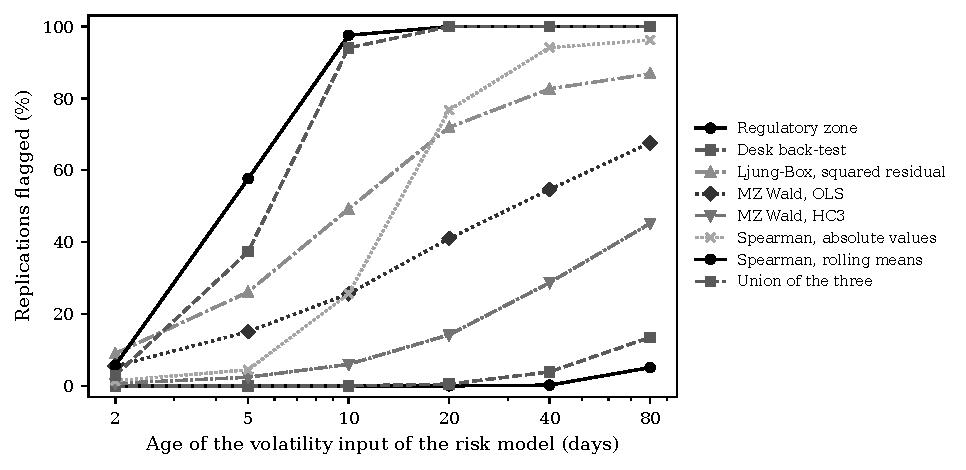
\includegraphics[width=0.86\linewidth]{power-by-lag}
\caption{Percent of 1,000 stale-volatility replications flagged by each detector against the age of the volatility input of the risk model in days (logarithmic axis), committed seeds; the regulatory zone and the desk back-test are near zero over the range where the rolling-mean statistic rises to 100\%.}
\label{fig:power-by-lag}
\end{figure}

\begin{figure}[htbp]
\centering
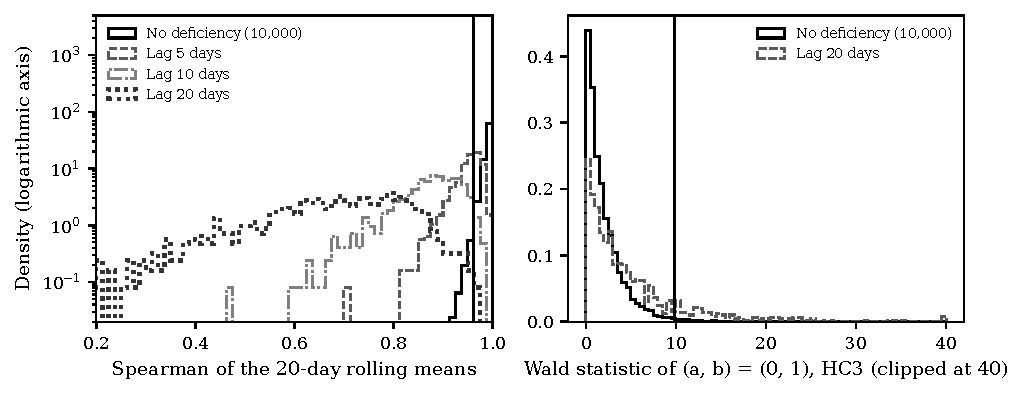
\includegraphics[width=\linewidth]{statistic-distributions}
\caption{Left: distribution of the rolling-mean Spearman statistic on the 10,000 null desk-years and on 1,000 stale-volatility desk-years at lags of 5, 10 and 20 days, with the 1\% critical value as a vertical line. Right: distribution of the HC3 Wald statistic on the null and at a lag of 20 days, clipped at 40, with its critical value.}
\label{fig:distributions}
\end{figure}

Figure~\ref{fig:distributions} shows why the two statistics differ: at a lag of 20 days the distribution of the rolling-mean statistic leaves the null almost entirely, whereas the distribution of the Wald statistic keeps most of its mass inside the null.

\subsection{A threshold-free comparison}
\label{sec:results-auc}

A detector's rate depends on its threshold; the area under the ROC curve does not.
Table~\ref{tab:auc} gives it for the nine statistics between the stale desks and the held-out null.
The rolling-mean statistic has the largest area at every lag: 0.976 at 5 days, 0.999 at 10 and 1.000 at 20 (0.9999 to 1.0000 at 20 days), against 0.837, 0.946 and 0.988 for the absolute-value statistic, 0.807, 0.925 and 0.980 for the Spearman correlation of the levels, and 0.699, 0.856 and 0.938 for the Ljung--Box statistic.
The Kolmogorov--Smirnov distance has 0.596, 0.680 and 0.785, and the Wald statistic with the HC3 covariance 0.549, 0.613 and 0.677.
The Spearman correlation of the levels has a large area, 0.980 at 20 days, while the regulatory zone flags nothing on this desk: the information is in the statistic, and the thresholds of the zone are what discard it.
Figure~\ref{fig:power-against-size} gives the power against the held-out false-alarm rate: at a lag of 10 days the rolling-mean statistic flags 86.2\% at 0.1\% size and 97.5\% at 1\%, while the Spearman correlation of the levels flags 1.3\% and 11.3\% at the same sizes.

\begin{table}[htbp]
\centering
\footnotesize
\caption{Area under the ROC curve of each statistic for separating 1,000 stale-volatility replications at the stated lag from the 1,000 held-out replications with no deficiency, with the 95\% percentile bootstrap interval (1,000 resamples); the area does not depend on any threshold, so it compares the statistics before calibration.}
\label{tab:auc}
\begin{tabular}{lccc}
\toprule
Statistic & Lag 5 days & Lag 10 days & Lag 20 days \\
\midrule
Spearman of 20-day rolling means & 0.976 (0.970--0.981) & 0.999 (0.998--1.000) & 1.000 (1.000--1.000) \\
Spearman of absolute values & 0.837 (0.818--0.855) & 0.946 (0.936--0.956) & 0.988 (0.983--0.991) \\
MZ Wald, HC3 & 0.549 (0.523--0.573) & 0.613 (0.590--0.639) & 0.677 (0.653--0.699) \\
MZ Wald, OLS covariance & 0.683 (0.659--0.706) & 0.749 (0.728--0.770) & 0.800 (0.780--0.819) \\
MZ Wald on squares & 0.580 (0.552--0.604) & 0.667 (0.640--0.690) & 0.786 (0.765--0.805) \\
Ljung--Box on squared residual & 0.699 (0.675--0.722) & 0.856 (0.837--0.872) & 0.938 (0.926--0.948) \\
Christoffersen conditional coverage & 0.541 (0.517--0.565) & 0.609 (0.582--0.634) & 0.692 (0.669--0.715) \\
KS distance (regulatory) & 0.596 (0.574--0.621) & 0.680 (0.658--0.703) & 0.785 (0.767--0.804) \\
Spearman of levels (regulatory) & 0.807 (0.788--0.827) & 0.925 (0.913--0.937) & 0.980 (0.974--0.985) \\
\bottomrule
\end{tabular}
\end{table}


\begin{figure}[htbp]
\centering
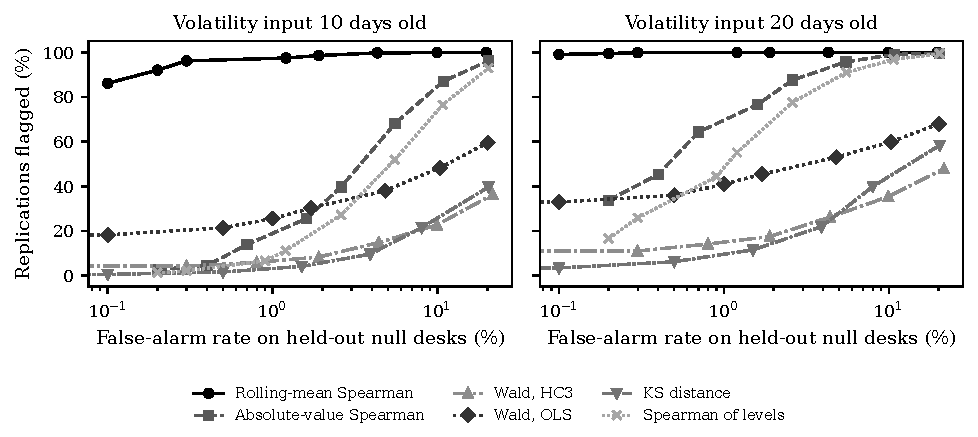
\includegraphics[width=\linewidth]{power-against-size}
\caption{Percent of stale-volatility replications flagged, at lags of 10 days (left) and 20 days (right), against the false-alarm rate on 1,000 held-out null desk-years (logarithmic axis), for sizes of 0.1\% to 20\% read from the 10,000 null desk-years; each curve is one statistic.}
\label{fig:power-against-size}
\end{figure}

\subsection{Defects the rank statistics cannot see}
\label{sec:results-misscale}

Table~\ref{tab:mis-scale} tests H5 on the no-deficiency desk with a constant defect planted in RTPL.
A mis-scale of 10\% in either direction gives a mean fitted slope of 1.111 or 0.909, the values $1/c$ of Proposition~\ref{prop:invariance}, and the Wald test flags 100.0\% of the replications; the regulatory zone flags 0.0\%, and the two rank statistics keep their false-alarm rates of 1.6\% and 1.2\%, unchanged by the rescaling.
A mis-scale of 20 or 25\% is flagged by the zone in 16.2\% and 8.4\%, and by the Wald test in 100.0\%.
A level error is seen by the rank statistics only when large: a shift of 0.1 standard deviations of the HPL is flagged by the Wald test in 100.0\%, by the zone in 18.2\%, by the absolute-value statistic in 26.0\% and by the rolling-mean statistic in 7.9\%, and a shift of 0.2 standard deviations by the zone in 97.3\% and by the rolling-mean statistic in 39.4\%.
H5 holds, and the table shows the role of the regression component: the two regression components, with either covariance, are the only detectors with full power against a constant mis-scale of 10\%.

\begin{table*}[htbp]
\centering
\scriptsize\setlength{\tabcolsep}{3pt}
\caption{Percent of 1,000 replications flagged, with the 95\% Wilson interval, when a constant mis-scale or a constant level error is planted in the risk-theoretical P\&L of the no-deficiency desk (case seed 13), with the mean Mincer--Zarnowitz slope of HPL on RTPL; every detector of the main comparison was run on these desks and the columns are the ones that respond (the desk back-test, the Christoffersen test and the recalibrated Spearman correlation of the levels flag at most 0.0\%, 0.8\% and 1.2\% in every row). The rank statistics are unchanged by a positive rescaling.}
\label{tab:mis-scale}
\resizebox{\textwidth}{!}{%
\begin{tabular}{lrccccccccc}
\toprule
Defect planted in the null desk & Mean slope & Zone & KS recal. & MZ OLS & MZ HC3 & MZ squares & LB sq. & Abs. Sp. & Roll Sp. & Union \\
\midrule
RTPL times 0.80 & 1.250 & 16.2 (14.0--18.6) & 100.0 (99.6--100.0) & 100.0 (99.6--100.0) & 100.0 (99.6--100.0) & 100.0 (99.6--100.0) & 34.3 (31.4--37.3) & 1.6 (1.0--2.6) & 1.2 (0.7--2.1) & 100.0 (99.6--100.0) \\
RTPL times 0.90 & 1.111 & 0.0 (0.0--0.4) & 34.9 (32.0--37.9) & 100.0 (99.6--100.0) & 100.0 (99.6--100.0) & 100.0 (99.6--100.0) & 11.3 (9.5--13.4) & 1.6 (1.0--2.6) & 1.2 (0.7--2.1) & 100.0 (99.6--100.0) \\
RTPL times 1.10 & 0.909 & 0.0 (0.0--0.4) & 12.1 (10.2--14.3) & 100.0 (99.6--100.0) & 100.0 (99.6--100.0) & 100.0 (99.6--100.0) & 11.4 (9.6--13.5) & 1.6 (1.0--2.6) & 1.2 (0.7--2.1) & 100.0 (99.6--100.0) \\
RTPL times 1.25 & 0.800 & 8.4 (6.8--10.3) & 100.0 (99.6--100.0) & 100.0 (99.6--100.0) & 100.0 (99.6--100.0) & 100.0 (99.6--100.0) & 39.6 (36.6--42.7) & 1.6 (1.0--2.6) & 1.2 (0.7--2.1) & 100.0 (99.6--100.0) \\
RTPL shifted by 0.1 sd of HPL & 1.000 & 18.2 (15.9--20.7) & 97.8 (96.7--98.5) & 100.0 (99.6--100.0) & 100.0 (99.6--100.0) & 2.8 (1.9--4.0) & 1.1 (0.6--2.0) & 26.0 (23.4--28.8) & 7.9 (6.4--9.7) & 100.0 (99.6--100.0) \\
RTPL shifted by 0.2 sd of HPL & 1.000 & 97.3 (96.1--98.1) & 100.0 (99.6--100.0) & 100.0 (99.6--100.0) & 100.0 (99.6--100.0) & 13.6 (11.6--15.9) & 0.7 (0.3--1.4) & 95.2 (93.7--96.4) & 39.4 (36.4--42.5) & 100.0 (99.6--100.0) \\
\bottomrule
\end{tabular}}
\end{table*}


\subsection{Size on desks that differ from the calibration null}
\label{sec:results-altnull}

Table~\ref{tab:alt-nulls} tests H3.
With the thresholds of the calibration null unchanged, the false-alarm rate of the union is 0.2\% when the volatility is less persistent (0.90) and 0.7\% when it is less dispersed (0.20), both at or below the stated size, and 0.3\% when the pricing noise is smaller.
It exceeds the stated size when the volatility is more persistent or more dispersed: 4.0\% (3.0 to 5.4\%) at a persistence of 0.995 and 6.2\% (4.9 to 7.9\%) at a dispersion of 0.50, where the absolute-value statistic alone has 8.5\% (6.9 to 10.4\%).
When the pricing noise is 30\% of the factor profit and loss the union flags 99.0\% (98.2 to 99.5\%) of desks with no deficiency, the absolute-value statistic 99.7\% and the rolling-mean statistic 63.5\%, while the Wald statistic with the HC3 covariance stays between 1.1 and 1.7\% and the Ljung--Box statistic at 1.1\% in every row.
H3 fails.
The rank statistics read the agreement of two scales, and a larger pricing noise is a real, if benign, loss of agreement between the pricing and the risk models; the calibration null has to be the desk's own, with its own noise, as Proposition~\ref{prop:size} requires through exchangeability.
Figure~\ref{fig:alt-null} gives the rates on a logarithmic scale.

\begin{table}[htbp]
\centering
\footnotesize
\renewcommand{\arraystretch}{1.1}
\caption{False-alarm rate in percent, over the 95\% Wilson interval, of each detector on 1,000 desk-years of a desk with no deficiency whose generator differs from the calibration null in one parameter, with every threshold taken unchanged from the calibration null; a rate above 1\% means the stated size does not transfer to that desk.}
\label{tab:alt-nulls}
\begin{tabular}{>{\raggedright\arraybackslash}p{4.4cm}cccc}
\toprule
Null desk & Zone & MZ HC3 & Abs. Sp. & Roll Sp. \\
\midrule
No deficiency, case seed 23 (the generator of the calibration null) & \begin{tabular}[t]{@{}c@{}}0.0\\(0.0--0.4)\end{tabular} & \begin{tabular}[t]{@{}c@{}}1.3\\(0.8--2.2)\end{tabular} & \begin{tabular}[t]{@{}c@{}}0.8\\(0.4--1.6)\end{tabular} & \begin{tabular}[t]{@{}c@{}}0.5\\(0.2--1.2)\end{tabular} \\ \addlinespace[0.8ex]
Volatility persistence 0.90 & \begin{tabular}[t]{@{}c@{}}0.0\\(0.0--0.4)\end{tabular} & \begin{tabular}[t]{@{}c@{}}1.7\\(1.1--2.7)\end{tabular} & \begin{tabular}[t]{@{}c@{}}0.0\\(0.0--0.4)\end{tabular} & \begin{tabular}[t]{@{}c@{}}0.0\\(0.0--0.4)\end{tabular} \\ \addlinespace[0.8ex]
Volatility persistence 0.995 & \begin{tabular}[t]{@{}c@{}}0.0\\(0.0--0.4)\end{tabular} & \begin{tabular}[t]{@{}c@{}}1.5\\(0.9--2.5)\end{tabular} & \begin{tabular}[t]{@{}c@{}}4.3\\(3.2--5.7)\end{tabular} & \begin{tabular}[t]{@{}c@{}}4.6\\(3.5--6.1)\end{tabular} \\ \addlinespace[0.8ex]
Volatility dispersion 0.20 & \begin{tabular}[t]{@{}c@{}}0.0\\(0.0--0.4)\end{tabular} & \begin{tabular}[t]{@{}c@{}}1.5\\(0.9--2.5)\end{tabular} & \begin{tabular}[t]{@{}c@{}}0.0\\(0.0--0.4)\end{tabular} & \begin{tabular}[t]{@{}c@{}}1.2\\(0.7--2.1)\end{tabular} \\ \addlinespace[0.8ex]
Volatility dispersion 0.50 & \begin{tabular}[t]{@{}c@{}}0.0\\(0.0--0.4)\end{tabular} & \begin{tabular}[t]{@{}c@{}}1.1\\(0.6--2.0)\end{tabular} & \begin{tabular}[t]{@{}c@{}}8.5\\(6.9--10.4)\end{tabular} & \begin{tabular}[t]{@{}c@{}}1.3\\(0.8--2.2)\end{tabular} \\ \addlinespace[0.8ex]
Pricing noise 5\% of factor P\&L & \begin{tabular}[t]{@{}c@{}}0.0\\(0.0--0.4)\end{tabular} & \begin{tabular}[t]{@{}c@{}}1.3\\(0.8--2.2)\end{tabular} & \begin{tabular}[t]{@{}c@{}}0.0\\(0.0--0.4)\end{tabular} & \begin{tabular}[t]{@{}c@{}}0.0\\(0.0--0.4)\end{tabular} \\ \addlinespace[0.8ex]
Pricing noise 30\% of factor P\&L & \begin{tabular}[t]{@{}c@{}}1.0\\(0.5--1.8)\end{tabular} & \begin{tabular}[t]{@{}c@{}}1.3\\(0.8--2.2)\end{tabular} & \begin{tabular}[t]{@{}c@{}}99.7\\(99.1--99.9)\end{tabular} & \begin{tabular}[t]{@{}c@{}}63.5\\(60.5--66.4)\end{tabular} \\ \addlinespace[0.8ex]
\bottomrule
\end{tabular}

\vspace{1.5ex}

\begin{tabular}{>{\raggedright\arraybackslash}p{4.4cm}ccc}
\toprule
Null desk & Union & LB sq. & MZ squares \\
\midrule
No deficiency, case seed 23 (the generator of the calibration null) & \begin{tabular}[t]{@{}c@{}}0.8\\(0.4--1.6)\end{tabular} & \begin{tabular}[t]{@{}c@{}}1.1\\(0.6--2.0)\end{tabular} & \begin{tabular}[t]{@{}c@{}}0.7\\(0.3--1.4)\end{tabular} \\ \addlinespace[0.8ex]
Volatility persistence 0.90 & \begin{tabular}[t]{@{}c@{}}0.2\\(0.1--0.7)\end{tabular} & \begin{tabular}[t]{@{}c@{}}1.1\\(0.6--2.0)\end{tabular} & \begin{tabular}[t]{@{}c@{}}1.5\\(0.9--2.5)\end{tabular} \\ \addlinespace[0.8ex]
Volatility persistence 0.995 & \begin{tabular}[t]{@{}c@{}}4.0\\(3.0--5.4)\end{tabular} & \begin{tabular}[t]{@{}c@{}}1.1\\(0.6--2.0)\end{tabular} & \begin{tabular}[t]{@{}c@{}}1.3\\(0.8--2.2)\end{tabular} \\ \addlinespace[0.8ex]
Volatility dispersion 0.20 & \begin{tabular}[t]{@{}c@{}}0.7\\(0.3--1.4)\end{tabular} & \begin{tabular}[t]{@{}c@{}}1.1\\(0.6--2.0)\end{tabular} & \begin{tabular}[t]{@{}c@{}}0.7\\(0.3--1.4)\end{tabular} \\ \addlinespace[0.8ex]
Volatility dispersion 0.50 & \begin{tabular}[t]{@{}c@{}}6.2\\(4.9--7.9)\end{tabular} & \begin{tabular}[t]{@{}c@{}}1.1\\(0.6--2.0)\end{tabular} & \begin{tabular}[t]{@{}c@{}}1.8\\(1.1--2.8)\end{tabular} \\ \addlinespace[0.8ex]
Pricing noise 5\% of factor P\&L & \begin{tabular}[t]{@{}c@{}}0.3\\(0.1--0.9)\end{tabular} & \begin{tabular}[t]{@{}c@{}}1.1\\(0.6--2.0)\end{tabular} & \begin{tabular}[t]{@{}c@{}}0.3\\(0.1--0.9)\end{tabular} \\ \addlinespace[0.8ex]
Pricing noise 30\% of factor P\&L & \begin{tabular}[t]{@{}c@{}}99.0\\(98.2--99.5)\end{tabular} & \begin{tabular}[t]{@{}c@{}}1.1\\(0.6--2.0)\end{tabular} & \begin{tabular}[t]{@{}c@{}}30.2\\(27.4--33.1)\end{tabular} \\ \addlinespace[0.8ex]
\bottomrule
\end{tabular}
\end{table}


\begin{figure}[htbp]
\centering
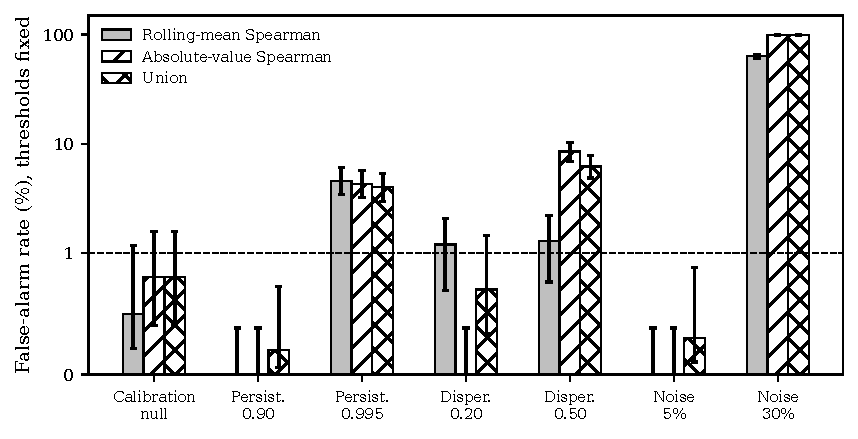
\includegraphics[width=0.88\linewidth]{alternative-nulls}
\caption{False-alarm rate in percent, on a symmetric logarithmic axis, of the rolling-mean statistic, the absolute-value statistic and the union on 1,000 desk-years with nothing planted whose generator differs from the calibration null in one parameter, with the 95\% Wilson interval and the 1\% stated size as a dashed line.}
\label{fig:alt-null}
\end{figure}

\subsection{The predictions}
\label{sec:results-hypotheses}

Table~\ref{tab:hypotheses} gives the outcome of each prediction.
H1 holds by a wide margin: the union flags the stale desk in 99.9\% of replications at a held-out false-alarm rate of 0.9\%, against the criterion of 30\% at a size of at most 1\% and a refutation bound of 10\%; the lower end of its interval, 99.4\%, is far above the criterion, and the size is not above 1\% beyond its sampling interval (0.5 to 1.7\%).
H2 holds in part.
The Wald statistic flags the wrong-correlation variant in 100.0\% of replications, as often as the Kolmogorov--Smirnov distance alone, and the desk with no deficiency at 0.8\%; it does not flag the missing-basis variant (0.9\% against 86.7\% for the distance), for the reason of Corollary~\ref{cor:noise}.
H3 fails, H4 holds and H5 holds, as shown above.

\begin{table*}[htbp]
\centering
\scriptsize
\caption{The five predictions of the experimental design, the criterion each was held to, the measured values on the committed bake or on the experiments of Section~\ref{sec:experimental-design}, and whether each held; H1 is the acceptance and refutation criterion fixed for the method before this evaluation and H2 the second clause of the research brief that proposed it.}
\label{tab:hypotheses}
\begin{tabular}{lp{4.8cm}p{6.2cm}l}
\toprule
Id & Prediction & Measured & Outcome \\
\midrule
H1 & \relax At a size of at most 1\%, the stale-volatility model is flagged in at least 30\% of replications; refuted below 10\% & \relax union 99.9 (99.4--100.0)\% at held-out size 0.9 (0.5--1.7)\%; regulatory zone 0.0\% & held \\
H2 & The Wald test flags wrong-correlation and missing-basis at least as often as the KS distance alone, and the no-deficiency desk at most at the stated rate & \relax wrong correlation 100.0\% against 100.0\%; missing basis 0.9\% against 86.7\%; no deficiency 0.8\% & held in part \\
H3 & \relax The false-alarm rate of the union stays at most 1\% on desks that differ from the calibration null & \relax 4.0\% (persistence 0.995), 6.2\% (dispersion 0.50), 99.0\% (pricing noise 30\%) & failed \\
H4 & The flag rate of the rolling-mean statistic rises with the age of the volatility input & \relax rates 5.7, 57.6, 97.5, 99.9, 100.0, 100.0\% at 2, 5, 10, 20, 40 and 80 days & held \\
H5 & The complement flags a constant mis-scale that the regulatory zone does not & \relax Wald 100.0\% against zone 0.0\% at a 10\% mis-scale & held \\
\bottomrule
\end{tabular}
\end{table*}


\subsection{Checks of the propositions}
\label{sec:results-theory}

Table~\ref{tab:theory-size} compares Proposition~\ref{prop:size} with the false-alarm rate of the critical value read from $N$ Gaussian null draws, repeated 2,000 to 20,000 times: the mean and the standard deviation agree with the proposition to the third significant figure (for $N=10{,}000$ and $p=1\%$, 1.012\% against 1.010\% and 0.100 against 0.100 points).
Table~\ref{tab:theory-loo} makes the check on the real null: each of the ten blocks of 1,000 null desk-years is flagged with the critical value calibrated on the other 9,000, and the mean over the ten folds is 1.01, 0.99 and 1.00\% for the Wald, absolute-value and rolling-mean statistics against 1.011\% predicted, with a standard deviation over folds of 0.31 to 0.35 points, close to the 0.31 points that a rate of 1\% on 1,000 desk-years carries.

\begin{table*}[htbp]
\centering
\footnotesize
\caption{Out-of-sample false-alarm rate, in percent, of the critical value that is the (k+1)-th most extreme of N independent standard normal null values: the mean and standard deviation that Proposition 1 gives and the values measured over the stated number of independent calibration draws.}
\label{tab:theory-size}
\begin{tabular}{rrrrrrrr}
\toprule
N & p (\%) & k & Draws & Mean, Prop. 1 & Mean, simulated & SD, Prop. 1 & SD, simulated \\
\midrule
100 & 5 & 5 & 20,000 & 5.941 & 5.931 & 2.341 & 2.352 \\
1,000 & 1 & 10 & 20,000 & 1.099 & 1.101 & 0.329 & 0.328 \\
1,000 & 5 & 50 & 20,000 & 5.095 & 5.090 & 0.695 & 0.695 \\
10,000 & 1 & 100 & 2,000 & 1.010 & 1.012 & 0.100 & 0.100 \\
10,000 & 0.333 & 33 & 2,000 & 0.340 & 0.338 & 0.058 & 0.058 \\
\bottomrule
\end{tabular}
\end{table*}


\begin{table}[htbp]
\centering
\footnotesize
\caption{Leave-one-block-out check of Proposition 1 on the real null: each of the ten blocks of 1,000 null desk-years is flagged with the critical value calibrated on the other 9,000; the table gives, in percent, the value Proposition 1 predicts for a calibration of 9,000 and the mean and standard deviation of the ten measured rates.}
\label{tab:theory-loo}
\begin{tabular}{>{\raggedright\arraybackslash}p{6.4cm}rrr}
\toprule
Statistic and size & Mean, Prop. 1 & Mean over 10 folds & SD over 10 folds \\
\midrule
\relax Wald, HC3 (1\% per statistic) & 1.011 & 1.010 & 0.354 \\
\relax Wald, HC3 (0.333\% per statistic) & 0.344 & 0.340 & 0.165 \\
\relax absolute-value Spearman (1\% per statistic) & 1.011 & 0.990 & 0.314 \\
\relax absolute-value Spearman (0.333\% per statistic) & 0.344 & 0.350 & 0.196 \\
\relax rolling-mean Spearman (1\% per statistic) & 1.011 & 1.000 & 0.320 \\
\relax rolling-mean Spearman (0.333\% per statistic) & 0.344 & 0.330 & 0.263 \\
\bottomrule
\end{tabular}
\end{table}


Table~\ref{tab:theory-slope-corr} and Figure~\ref{fig:theory-check} compare Propositions~\ref{prop:slope} and~\ref{prop:rolling} with simulation.
On windows of 100,000 days the simulated slope equals Equation~\eqref{eq:slope} to within 1.2 standard errors at every lag (0.9603 against 0.9601 at 20 days) and the simulated correlation of the rolling means equals Equation~\eqref{eq:rolling-corr} to within 0.006 (0.8084 $\pm$ 0.0014 against 0.8054 at 20 days; 0.6021 $\pm$ 0.0025 against 0.5969 at 40).
On the 250-day windows of the desk the mean correlation is lower, 0.6946 $\pm$ 0.0023 at 20 days in the noise-free model and 0.6908 on the committed desks with their pricing noise, and the mean slope is above the closed form by 0.003 at 20 days (0.9633 against 0.9601) and by 0.016 at 80 days, which is the small-sample bias of a ratio of sample moments of a persistent process.
The closed forms are population quantities, the 250-day desk is a sample of them, and the thresholds are calibrated on the sample law, so the decision never depends on the population value.

\begin{table}[htbp]
\centering
\footnotesize
\renewcommand{\arraystretch}{1.1}
\caption{The Mincer--Zarnowitz slope and the Pearson correlation of the 20-day rolling means of the absolute series at each lag of the volatility input: the closed forms of Propositions 2 and 3, the mean over 1,000 C13 desk-years of 250 days (with its standard error, and for the slope its standard deviation over desk-years), and an independent simulation of the noise-free model on windows of 100,000 and of 250 days (mean and standard error over 20 and 4,000 windows). The first panel is the slope, the second the correlation.}
\label{tab:theory-slope-corr}
\begin{tabular}{rcccc}
\toprule
Lag & \shortstack{Closed\\form} & \shortstack{100,000-day\\windows} & \shortstack{C13\\mean} & \shortstack{C13\\sd} \\
\midrule
0 & 1.0000 & $1.0000\pm0.0000$ & $1.0002\pm0.0002$ & 0.0069 \\ \addlinespace[0.8ex]
2 & 0.9952 & $0.9951\pm0.0001$ & $0.9955\pm0.0004$ & 0.0128 \\ \addlinespace[0.8ex]
5 & 0.9883 & $0.9885\pm0.0002$ & $0.9882\pm0.0006$ & 0.0202 \\ \addlinespace[0.8ex]
10 & 0.9778 & $0.9776\pm0.0002$ & $0.9788\pm0.0010$ & 0.0310 \\ \addlinespace[0.8ex]
20 & 0.9601 & $0.9603\pm0.0003$ & $0.9633\pm0.0016$ & 0.0508 \\ \addlinespace[0.8ex]
40 & 0.9344 & $0.9346\pm0.0005$ & $0.9426\pm0.0026$ & 0.0836 \\ \addlinespace[0.8ex]
80 & 0.9065 & $0.9063\pm0.0009$ & $0.9228\pm0.0042$ & 0.1312 \\ \addlinespace[0.8ex]
\bottomrule
\end{tabular}

\vspace{1.5ex}

\begin{tabular}{rcccc}
\toprule
Lag & \shortstack{Closed\\form} & \shortstack{100,000-day\\windows} & \shortstack{250-day\\windows} & \shortstack{C13\\mean} \\
\midrule
0 & 1.0000 & $1.0000\pm0.0000$ & $1.0000\pm0.0000$ & $0.9942\pm0.0002$ \\ \addlinespace[0.8ex]
2 & 0.9959 & $0.9960\pm0.0000$ & $0.9932\pm0.0001$ & $0.9874\pm0.0003$ \\ \addlinespace[0.8ex]
5 & 0.9800 & $0.9802\pm0.0001$ & $0.9666\pm0.0003$ & $0.9610\pm0.0007$ \\ \addlinespace[0.8ex]
10 & 0.9333 & $0.9340\pm0.0005$ & $0.8909\pm0.0009$ & $0.8866\pm0.0018$ \\ \addlinespace[0.8ex]
20 & 0.8054 & $0.8084\pm0.0014$ & $0.6946\pm0.0023$ & $0.6908\pm0.0044$ \\ \addlinespace[0.8ex]
40 & 0.5969 & $0.6021\pm0.0025$ & $0.4284\pm0.0038$ & $0.4203\pm0.0076$ \\ \addlinespace[0.8ex]
80 & 0.3717 & $0.3732\pm0.0039$ & $0.2286\pm0.0050$ & $0.2089\pm0.0099$ \\ \addlinespace[0.8ex]
\bottomrule
\end{tabular}
\end{table}


\begin{figure}[htbp]
\centering
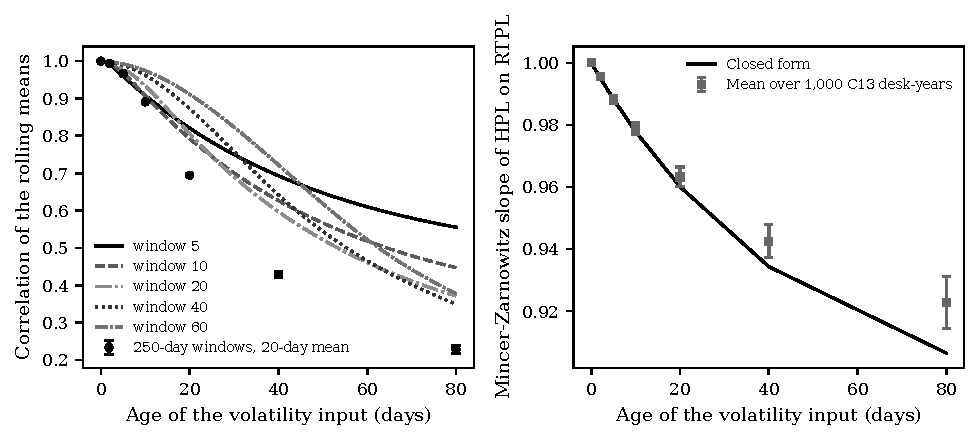
\includegraphics[width=\linewidth]{theory-check}
\caption{Left: the closed-form correlation of the rolling means against the age of the volatility input, for five windows, with the mean and twice the standard error of the simulated 250-day windows for the 20-day mean. Right: the closed-form regression slope of Proposition~\ref{prop:slope} against the mean fitted slope over 1,000 C13 desk-years with twice its standard error.}
\label{fig:theory-check}
\end{figure}
